\section{\textit{Command-Query Responsibility Segregation}}

\textit{Command-Query Responsibility Segregation} (CQRS) merupakan sebuah \textit{pattern} yang memisahkan operasi \textit{read} dan \textit{update} untuk sebuah media penyimpanan data. Dalam pemodelan data, seringkali model data yang sama digunakan untuk operasi pembacaan dan pembaruan. Meskipun begitu, seringkali kedua operasi tersebut memiliki kebutuhan yang berbeda. CQRS menggunakan model data yang berbeda untuk kedua operasi yang berbeda. Selain itu, beban pekerjaan untuk kedua operasi tersebut seringkali asimetris dan memiliki kebutuhan kinerja dan \textit{scaling} yang berbeda \parencite{msCQRS}.

\textit{Command} berupa perintah yang berfokus pada pekerjaan, seperti memesan kamar hotel dibandingkan dengan ubah status reservasi suatu kamar menjadi \textit{reserved}. Dengan pendekatan ini, \textit{command} dapat diproses secara asinkron.

\begin{figure}[ht]
    \centering
    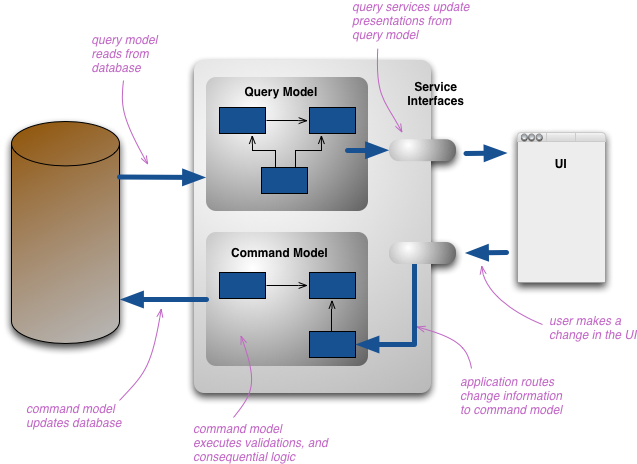
\includegraphics[width=0.8\textwidth]{resources/chapter-2/cqrs.png}
    \caption{\textit{CQRS Illustration} \parencite{fwCQRS}}
    \label{fig:cqrs-illustration}
\end{figure}

Pendekatan ini memungkinkan pemisahan data untuk operasi pembacaan dan data untuk operasi pembaruan. Pembacaan data dapat dilakukan pada skema atau basis data yang telah dioptimalkan untuk operasi tersebut, seperti menyimpan data di memori, \textit{materialized view}, atau pun yang lainnya.

Pendekatan ini memungkinkan \textit{scaling} secara independen dan \textit{separation of concerns}. Meskipun begitu, implementasinya bisa menjadi kompleks dan apabila basis data untuk operasi pembacaan dan pembaruan berbeda, data menjadi \textit{eventual consistent}.